\documentclass[12pt, a4paper]{article}

\usepackage[T2A]{fontenc}
\usepackage[utf8]{inputenc}
\usepackage[english,russian]{babel}
\usepackage[left = 1.5 cm, right = 1.5 cm, top = 2cm, bottom = 2 cm, bindingoffset = 0 cm]{geometry}
\usepackage{amsmath,amsfonts,amssymb,amsthm,mathtools}
\usepackage{wasysym}
\usepackage{float}

\usepackage{tikz}

\usepackage{graphicx}
\graphicspath{{pictures/}}
\DeclareGraphicsExtensions{.pdf,.png,.jpg}

\usepackage{alltt}

\begin{document}
\begin{titlepage}
\newpage

\begin{center}
Министерство образования и науки Российской Федерации \\
Федеральное государственное автономное образовательное
учреждение высшего образования \\
Национальный исследовательский Нижегородский государственный
университет им. Н.И. Лобачевского \\
Институт информационных технологий, математики и механики \\
\end{center}

\vspace{12em}

\begin{center}
\textsc{\textbf{Отчёт по лабораторной работе}}\\
\textsc{\textbf{Численные методы исследования динамических систем с помощью пакета MatLab}}
\end{center}

\vspace{14em}



\newbox{\lbox}
\savebox{\lbox}{\hbox{Барабаш Н. В.}}
\newlength{\maxl}
\setlength{\maxl}{\wd\lbox}
\hfill\parbox{11cm}{
\hspace*{5cm}\hspace*{-2cm} \textbf{Выполнил:} студент группы 381803-1 \\
\hspace*{5cm}\hspace*{-2cm} Петров Павел \\
\hspace*{5cm}\hspace*{-2cm} \textbf{Проверил:} научный сотрудник \\
\hspace*{5cm}\hspace*{-2cm} лаборатории динамического хаоса \\
\hspace*{5cm}\hspace*{-2cm} кафедры ТУиДС \\
\hspace*{5cm}\hspace*{-2cm} Казаков А. О. \\
\\
}


\vspace{\fill}
\vspace{\fill}

\begin{center}
Нижний Новгород \\2021
\end{center}

\end{titlepage}

\section{Отображение параболы}
Рассмотрим отображение параболы $x_{n+1} = 1 - a x^2_{n}$, где $a$ - некоторый параметр.
\newline
Найдём координаты неподвижных точек.
\[ \bar x = 1 - a \bar x^2 \]
\[ a \bar x^2 + \bar x - 1 = 0 \]
\[ \bar x_{1,2} = \frac{-1 \pm \sqrt{1 + 4a}}{2a}\]
Видим, что неподвижные точки существуют при $ a \geq -0,25$.
Выясним происходит ли удвоение периода (т.е. равен ли мультипликатор $\mu$ -1).
\[ \mu = (1 - ax^2)' = -2ax = 1 \mp \sqrt{1 + 4a} = -1 \]
\[ 2 = \pm \sqrt{1 + 4a}\]
Видим, что при $a = \frac{3}{4}$ точка $ \bar x = \frac{-1 + \sqrt{1 + 4a}}{2a} $ , которая была устойчива, теряет такую характеристику и рождает цикл периода 2. Другая же точка будет всегда неустойчива, поскольку при $a \geq -0.25$ её мультипликатор $\mu \geq 1$.
\newline
Вычислим координаты точек периода 2.
\[ \begin{cases} 
		x_2 = 1 - ax^2_1 \\
		x_1 = 1 - ax^2_2 \\
		x_1 \neq x_2
   \end{cases}
\]
Вычтем из первого уравнения второе.
\[ (x_2 - x_1)(1 - a(x_2 + x_1)) = 0 \]
\[ x_1 + x_2 = \frac{1}{a} \]
Сложим первые два уравнения системы.
\[ \frac{1}{a} = 2 - a(x^2_1 + x^2_2) \]
\[ x^2_1 + x^2_2 = \frac{1}{a^2} - 2x_1 x_2\]
\[ \frac{1}{a} = 2 - \frac{1}{a} + 2ax_1 x_2 \]
\[ x_1 x_2 = \frac{1 - a}{a^2} \]
Имеем следующую систему:
\[
	\begin{cases}
		x_1 + x_2 = \frac{1}{a} \\
		x_1 x_2 = \frac{1 - a}{a^2}
	\end{cases}
\]
Соответствующее её квадратное уравнение и его корни имеют вид:
\[ x^2 - \frac{1}{a} x + \frac{1 - a}{a^2} = 0 \]
\[ x_{1,2} = \frac{1 \pm \sqrt{4a - 3}}{2a} \]
Видим, что точки цикла периода два существуют при $a \geq \frac{3}{4}$, что было выяснено ранее.
\subsection{Аналитически построить график зависимости координат неподвижных точек от параметра а}
Используя приведённые выше выкладки, аналитически построим часть графика зависимости координат неподвижных точек от параметра.
\begin{figure}[H]
	\center{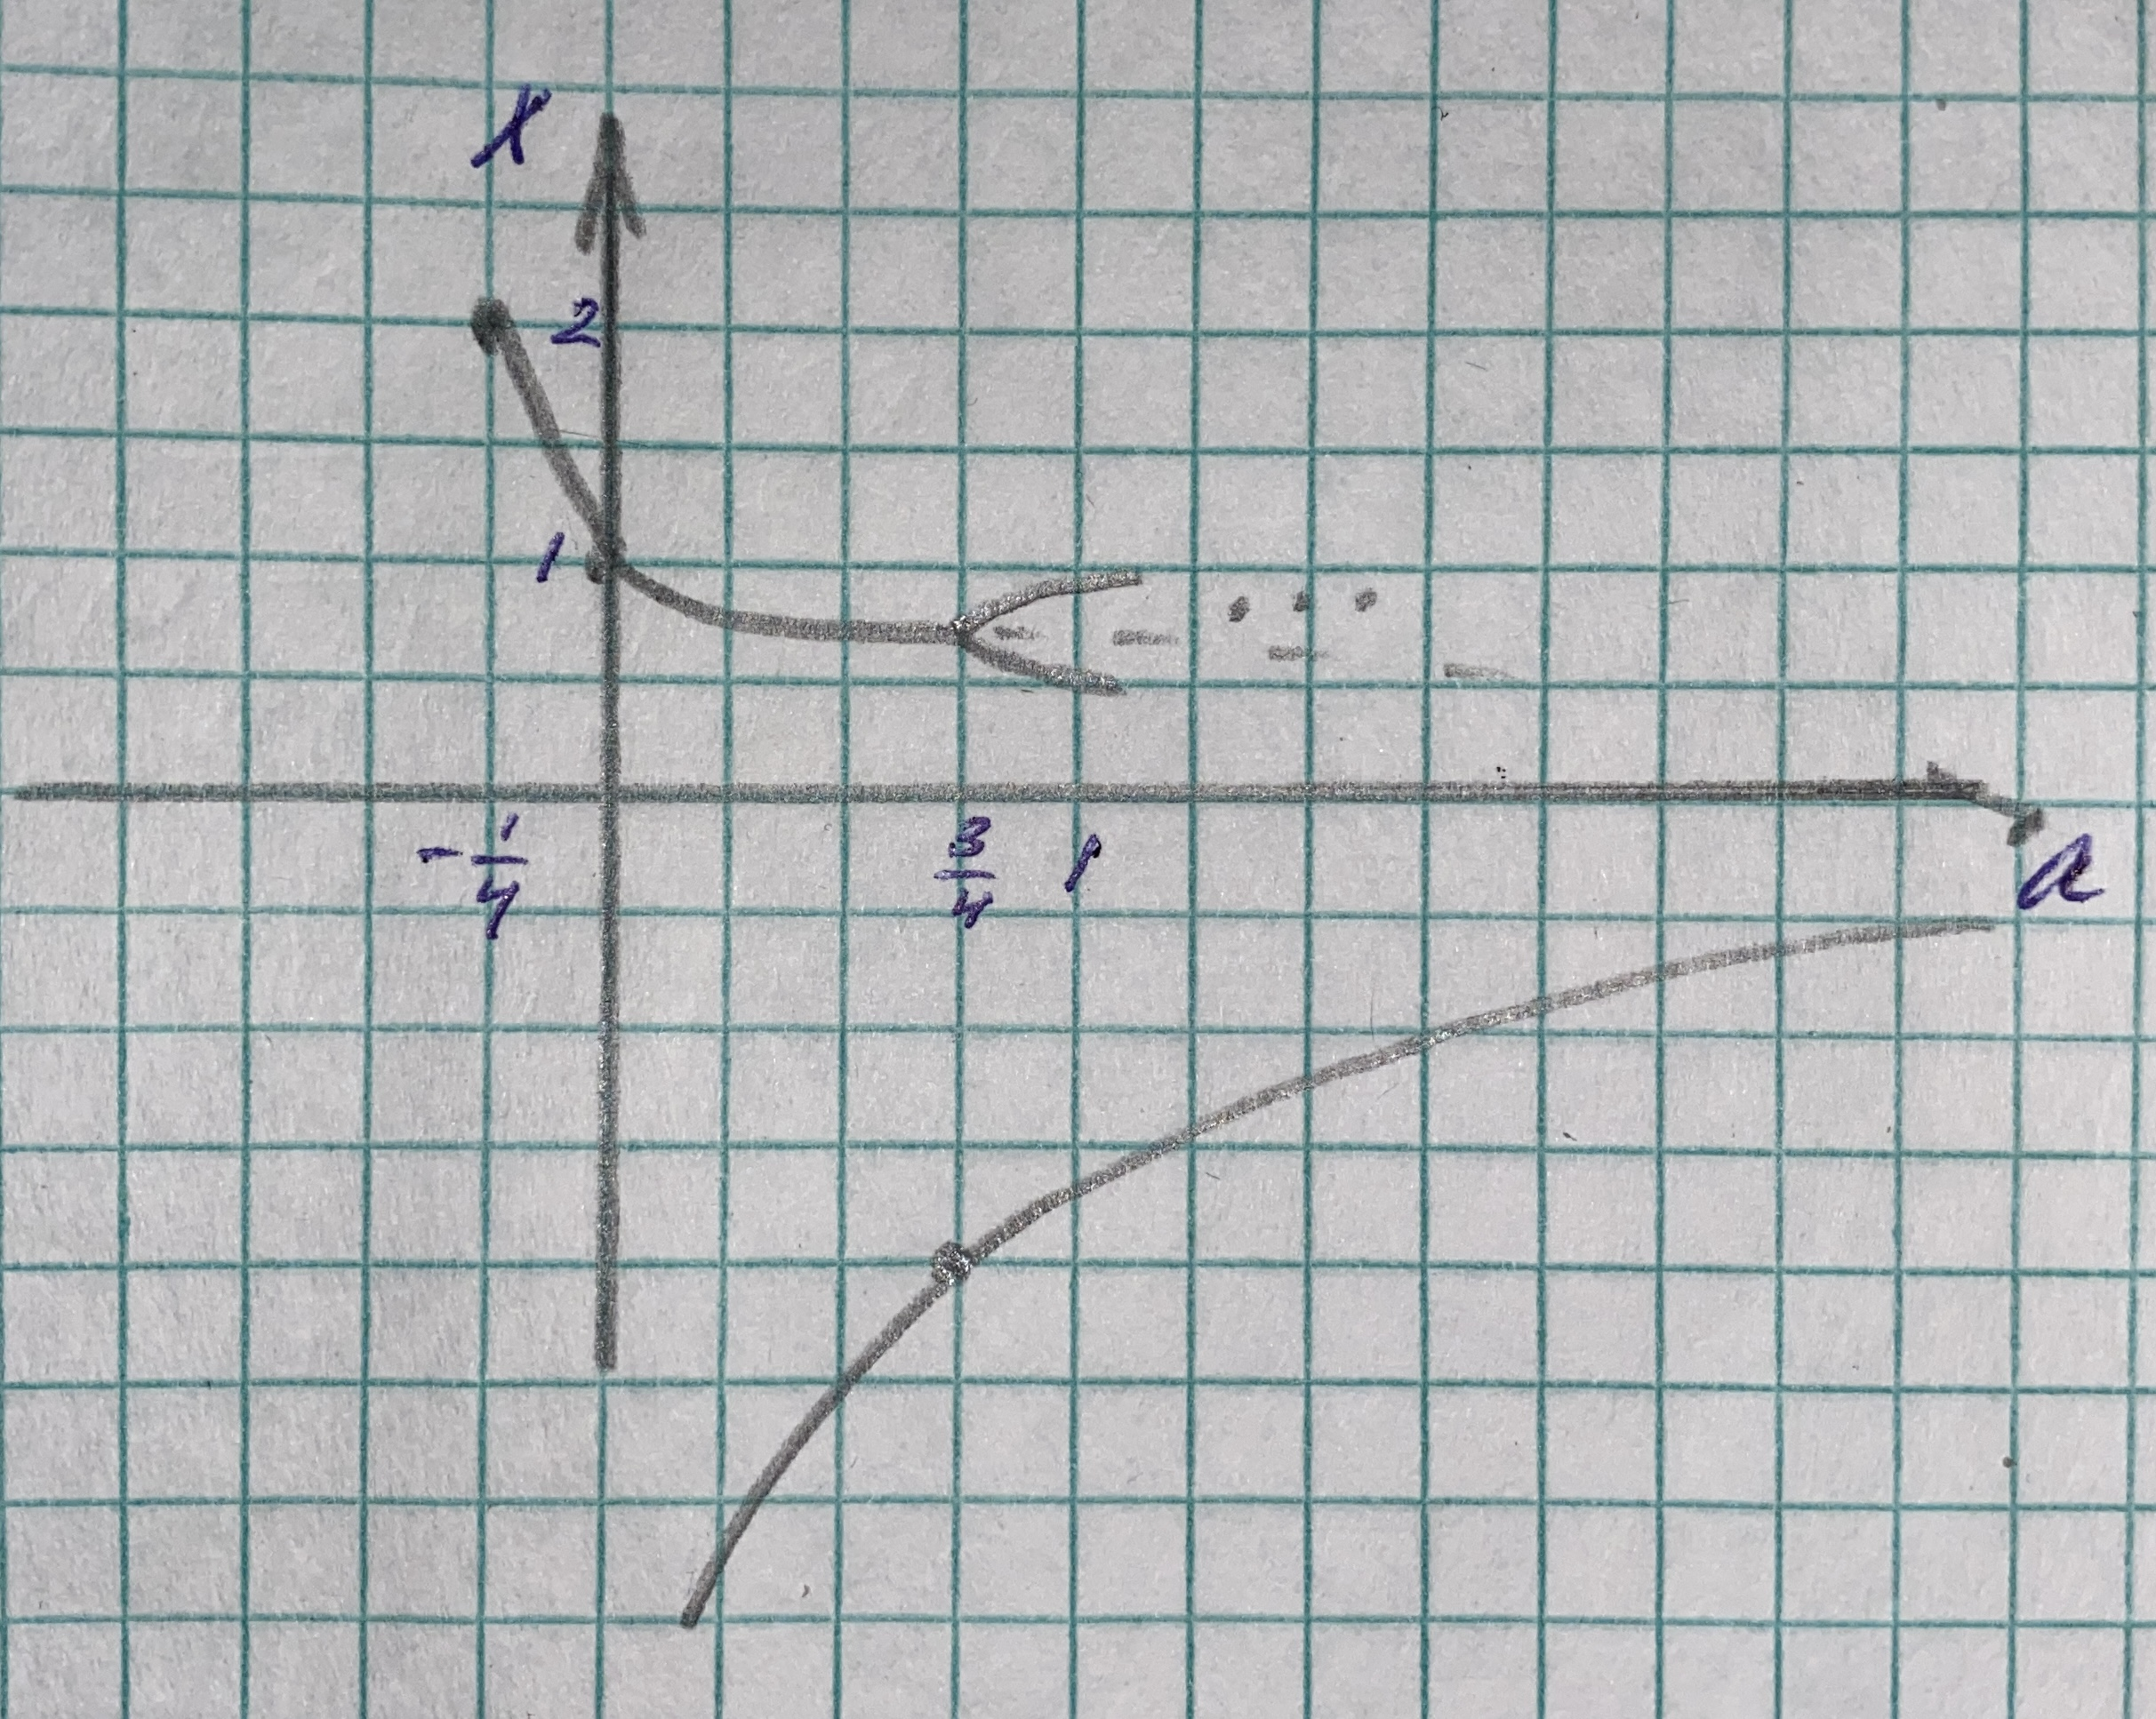
\includegraphics[scale=0.1]{feigan}}
	\caption{Часть аналитически построенного дерева Фейгенбаума}
\end{figure}

\subsection{Численно построить дерево Фейгенбаума}
Дерево Фейгенбаума для данного отображения строилось следующим образом. Выбиралась начальная точка с координатой 0.1 и параметр 0.2. С помощью orbit simulation находилась неподвижная точка, которая далее протягивалась по параметру a. В результате находился параметр, при котором происходило удвоение периода. Далее эта точка выбиралась и протягивалась с помощью FP curve x2. В результате находился параметр, при котором происходит очередная бифуркация удвоения периода и рождается устойчивый цикл периода 4. Эти параметры запоминались, далее выбирались промежуточные значения между ними и с помощью orbit simulation находились координаты неподвижных точек циклов периода 2, 4 и 8. Поочерёдно выбирая эти точки, выставляя параметр iteration равным циклу, которому соответствует неподвижная точка, и выбирая FP curve x1, выстраивалось дерево.
\begin{figure}[H]
	\center{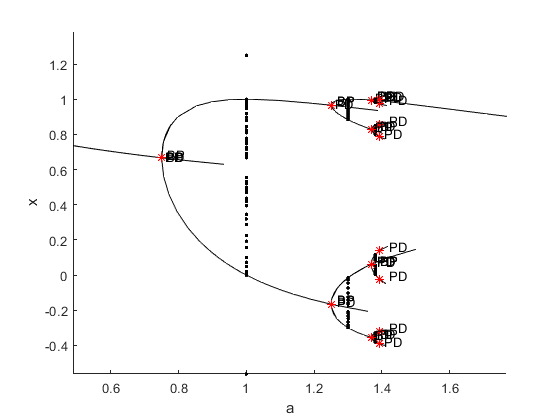
\includegraphics[scale=0.6]{ParMFeigTree1}}
	\caption{Численно построенное дерево Фейгенбаума}
\end{figure}

\section{Отображение Эно}
Рассмотрим отображение вида:
\begin{equation*}
	\begin{cases}
		x_{n + 1} = y_n \\
		y_{n + 1} = \lambda - bx_n - y^2_n
	\end{cases}
\end{equation*}
\subsection{Аналитически построим бифуркационную диаграмму отображения Эно}
Найдём неподвижные точки отображения:
\begin{equation*}
	\begin{cases}
		x = y \\
		y = \lambda - bx + y^2
	\end{cases}
\end{equation*}

\[ x = \lambda - bx + x^2 \]
\[ x^2 - (1 + b)x + \lambda = 0 \]
\[ \bar x_{1,2} = \frac{1 + b}{2} \pm \frac{\sqrt{(1 + b)^2 - 4\lambda}}{2} \]

Найдём характеристический многочлен системы:
\begin{equation*}
	\begin{vmatrix}
		-\mu & 1 \\
		-b & 2y  - \mu
	\end{vmatrix}
	= \mu^2 - 2y\mu + b = 0
\end{equation*}

Найдём бифуркационные кривые:
\newline
$\mu = 1$ - седло-узловая бифуркация:
\[ 1 - 2y + b = 0 \]
\[ y = \frac{1 + b}{2} \]
\[ \bar y_{1,2} = \bar x_{1,2} \]
\[ \frac{1 + b}{2} = \frac{1 + b}{2} \pm \frac{\sqrt{(1 + b)^2 - 4\lambda}}{2} \]
\[ (1 + b)^2 - 4\lambda = 0 \]
\[ \lambda = \frac{(1 + b)^2}{4} \]
\newline
$\mu = -1$ - бифуркация удвоения периода:
\[ 1 + 2y + b = 0 \]
\[ y = -\frac{1 + b}{2} \]
\[ \bar y_{1,2} = \bar x_{1,2} \]
\[ -\frac{1 + b}{2} = \frac{1 + b}{2} \pm \frac{\sqrt{(1 + b)^2 - 4\lambda}}{2} \]
\[ -2(1 + b) = \pm \sqrt{(1 + b)^2 - 4\lambda} \]
Рассматривая разные знаки выражения левой части, получим один и тот же результат.
\[ 4(1 + b)^2 = (1 + b)^2 - 4\lambda \]
\[ \lambda = -\frac{3}{4} (1 + b)^2 \]
Нарисуем бифуркационную диаграмму в плоскости $(b. \lambda) $.

\subsection{Построить бифуркационную диаграмму в Matcont}
\begin{figure}[H]
	\center{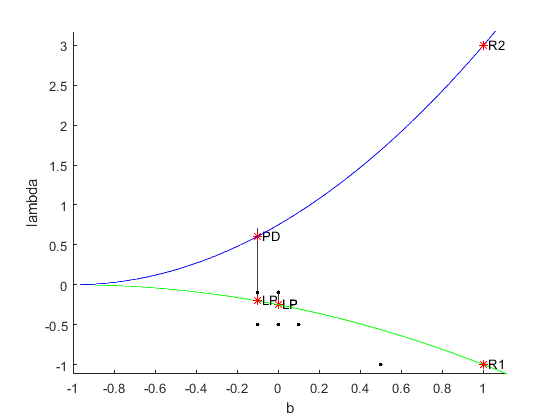
\includegraphics[scale=0.7]{HenonBifDiag1}}
	\caption{Бифуркационная диаграмма отображения Эно}
\end{figure}

Для построения бифуркационной диаграммы изначально выбирается точка $90.1; 0.2)$ и параметры $(b, \lambda) = -0.1)$. Выбирается orbit simulation и находится неподвижная точка отображения. С помощью этой точки, протягивая по параметру $b$ находим limit point, которую протягиваем по двум параметрам. Аналогично, протягивая неподвижную точку по $\lambda$ находим кривую бифуркации удвоения периода. Протягиваем её по двум параметрам как PD-curve x1, затем, выбирая FP-curve x2, протягиваем по параметру $\lambda$ и натыкаемся на ещё одну кривую бифуркации удвоения периода. Проделываем аналогичную процедуру, что и для устойчивой точки периода 1. Выбирая FP-curve x2, натыкаемся на очередную кривую бифуркации удвоения периода, которую с помощью PD-curve x1 протягиваем по двум параметрам. Таким образом получаем бифуркационные кривые для устойчивых точек периода 2 и 4.
\subsection{Построить бифуркационные кривые для устойчивых точек периода 2 и 4}
\begin{figure}[H]
	\center{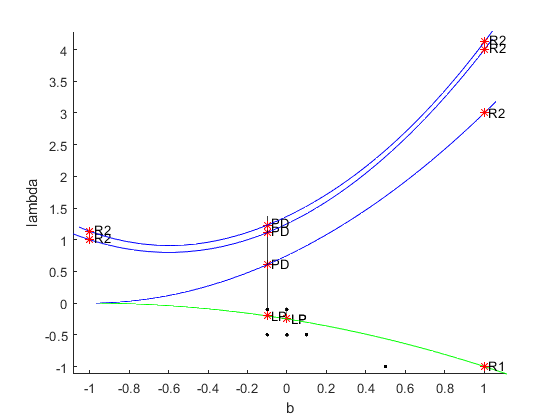
\includegraphics[scale=0.7]{HenonBifDiag2}}
	\caption{Бифуркационные кривые устойчивых точек периода 2 и 4}
\end{figure}
\section{Отображение Мира}
Рассмотрим отображение вида:
\begin{equation*}
	\begin{cases}
		x_{n + 1} = 1 - \lambda y^2_n + b x_n \\
		y_{n + 1} = x_n
	\end{cases}
\end{equation*}

\subsection{Аналитически построить бифуркационную диаграмму для неподвижных точек}
Найдём неподвижные точки отображения:
\begin{equation*}
	\begin{cases}
		x = 1 - \lambda y^2 + b x \\
		y = x
	\end{cases}
\end{equation*}

\[ \lambda x^2 + (1 - b)x - 1 = 0 \]
\[ \bar y_{1,2} = \bar x_{1,2} = - \frac{1 - b}{2 \lambda} \pm \frac{\sqrt{(1 - b)^2 + 4 \lambda}}{2 \lambda} \]

Найдём характеристический многочлен системы:
\begin{equation*}
	\begin{vmatrix}
		b - \mu & -2y\lambda \\
		1 & 0 - \mu
	\end{vmatrix} =
	\mu^2 - b\mu + 2y\lambda = 0
\end{equation*}

Найдём бифуркационные кривые:
\newline
$\mu = 1$ - седло-узловая бифуркация:
\[ 1 - b + 2 \bar y \lambda = 0 \]
\[ \bar y = - \frac{1 - b}{2\lambda} \]
\[ \bar y_{1,2} = \bar x_{1, 2} \]
\[ - \frac{1 - b}{2\lambda} =  - \frac{1 - b}{2 \lambda} \pm \frac{\sqrt{(1 - b)^2 + 4 \lambda}}{2 \lambda} \]
\[ \frac{\sqrt{(1 - b)^2 + 4 \lambda}}{2 \lambda} = 0 \] 
\[ (1 - b)^2 + 4 \lambda = 0 \]
\[ \lambda = -\frac{(1 - b)^2}{4} \] 
\newline
$\mu = -1$ - бифуркация удвоения периода:
\[ 1 + b + 2 \bar y \lambda = 0 \]
\[ \bar y = - \frac{1 + b}{2\lambda} \]
\[ \bar y_{1,2} = \bar x_{1, 2} \]
\[ - \frac{1 + b}{2\lambda} =  - \frac{1 - b}{2 \lambda} \pm \frac{\sqrt{(1 - b)^2 + 4 \lambda}}{2 \lambda} \]
\[ -2b = \pm \sqrt{(1 - b)^2 + 4 \lambda} \]
Рассмотрев случаи $b \geq 0$ и $b < 0$, придём к одной и той же формуле.
\[ 4b^2 = 1 - 2b + b^2 + 4\lambda \]
\[ \lambda = \frac{3b^2 + 2b - 1}{4} = \frac{(b + 1)(3b - 1)}{4} \]
\newline
$\mu = e^{i\varphi}$ - бифуркация Неймарка-Сакера:
\newline 
Подставив в характеристическое уравнения получим:
\[ 2\lambda \bar y = 1 \]
\[ \frac{1}{2\lambda} = - \frac{1 - b}{2 \lambda} \pm \frac{\sqrt{(1 - b)^2 + 4 \lambda}}{2 \lambda} \]
\[ 2 + b = \pm \sqrt{(1 - b)^2 + 4 \lambda} \]
Рассматривая разные случая знака выражения слева, получим один и тот же результат:
\[ b^2 - 4b + 4 = 1 - 2b + b^2 + 4\lambda \]
\[ \lambda = \frac{3 - 2b}{4} \]
Изобразим получившиеся кривые на плоскости.

\end{document}